\section{Preliminaries: Paths, Routes, and Policy}\label{sec:definitions}

Before introducing the correctness properties themselves, we first
introduce some basic terminology for routing.  We explain these terms in
the context of Internet routing and BGP.  We first define paths and
routes in terms of a graph $G = (V,E)$, where the nodes in $V = \{v_1,
\ldots, v_N\}$ correspond to IP-level nodes (\ie, routers and end hosts)
and the edges in $E$ corresponds to IP-level links between those nodes.

\subsection{Paths and Routes}

We now define two basic terms---path and route---and explain how they
are related.
% We first define these terms generally.  Then,
%we discuss them using Internet routing as an example.

\begin{defn}[Path]\label{defn:rl:path}
A {\em path} is a sequence of nodes $P = (v_0, \ldots, v_n)$, where $v_i
\in G$ for all $0 \leq i \leq n$.
\end{defn}

\noindent
The definition of a path does not constrain how the sequence of nodes is
actually constructed.  As such, a path might represent a sequence of
directly connected IP-layer nodes or endpoints of a tunnel.\footnote{A
{\em tunnel} is a sequence of nodes that all forward packets to some
intermediate node (\ie, the tunnel's ``exit''), rather than the
ultimate destination.  A tunnel may be implemented by a variety of
mechanisms, such as IP-in-IP encapsulation~\cite{rfc2784}, Multiprotocol
Label Switching (MPLS)~\cite{davie:mplsbook,mpls-wg}, etc.}
Note that 
deleting some nodes from a path still results in a path.  
%For example, a path
%that is a sequence of tunnel endpoints can be constructed by taking the
%corresponding IP-layer path and deleting all nodes but the tunnel
%endpoints. A path could even even represent AS-level hops if it only
%included one IP-level hop per AS.

In contrast to a path, a route is {\em information} that allows nodes in
$G$ to construct paths to {\em destinations}.  The {\em destination} $d$
may refer either to a single node or a group of nodes (named, for
example, by an IP prefix).  The purpose of a routing protocol is to
propagate routes for destinations.  Collectively, the routes to $d$ that
the nodes in $G$ ultimately select define the {\em path} from any node
in $G$ to that destination.  All of our definitions presume that the
handle for a destination, $d$, cannot be manipulated (\eg, our
definitions do not consider the effects of IP prefix
aggregation~\cite{rfc1519,rfc1518}). 

\begin{defn}[Route]\label{def:route}
A {\em route} is a mapping $(d \rightarrow v_i)$, where $d$ is a
destination, and $v_i \in G$ is a node en route to the destination
$d$.  
\end{defn}
\noindent
We say that $v_i\in d$ if the destination $d$ includes $v_i$.  A route
$(d \rightarrow v_i)$ received by $v_j$ indicates that, if $v_j$ has a
packet to send to some node at destination $d$, it can forward that
packet to $v_i$, which in turn ought to have a route to $d$ (whereupon
this process repeats until the data reaches $d$).  One can think of a
route $(d \rightarrow v_i)$ being used at node $v_j$ as {\em inducing}
a path, $(v_j, \ldots, v_i)$, where either $v_j$ and $v_i$ are directly
connected or where the actual nodes along that path segment are
determined by the connectivity between those nodes, as established by the
IGP or using tunnels.  We will formalize the notion of induced paths in
Section~\ref{sec:consistency}.

Note that Definition~\ref{def:route} can apply to any routing protocol,
not just to BGP.  In an IGP, the node $v_i$ is typically the router that is
immediately connected at the IP layer.  In BGP, however, (particularly
in iBGP) the next hop may be several IP-layer hops away.  In
BGP, a node that receives a route $(d \rightarrow v)$ but is not
directly connected to $v$ must rely on the IGP for reachability to $v$.

\subsection{Induced Paths and Consistent Paths}\label{sec:consistency}

We can think of paths as being {\em induced} by routes.  That is, while
there exist many sequences of nodes between any node $v_0$ and a node in some
destination $d$, the path that traffic will actually take from $v_0$ en
route to $d$ is determined by the routes that the nodes in $G$ select.
In many routing protocols, including BGP, no single node has knowledge
about the entire sequence of nodes that traffic traverses en route to
$d$; rather, the
nodes that the routes select collectively {\em induce} a path to $d$.  We are
interested in making statements about those induced paths.  We now
formalize the concept of induced paths and describe a special class of
induced paths called {\em consistent paths}.

\begin{figure}
\centering
\begin{psfrags}
\psfrag{vi}{ $v_1$}
\psfrag{vid}{{\small $v_n \in d$}}
\psfrag{vi1}{$v_{i-1}$}
\psfrag{v0}{$v_0$}
\psfrag{v1}{$v_1$}
\psfrag{p1}{$P_{v_0}(r_{v_0}(v_i))$}
\psfrag{p2}{$P_{v_1}(r_{v_1}(d))$}
\psfrag{p3}{$P_{v_0}(r_{v_0}(d))$}
\resizebox{0.5\textwidth}{!}{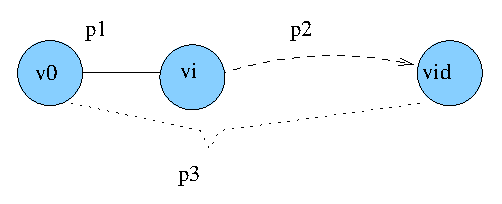
\includegraphics{rlogic/figures/induced_path1.eps}}
\end{psfrags}
%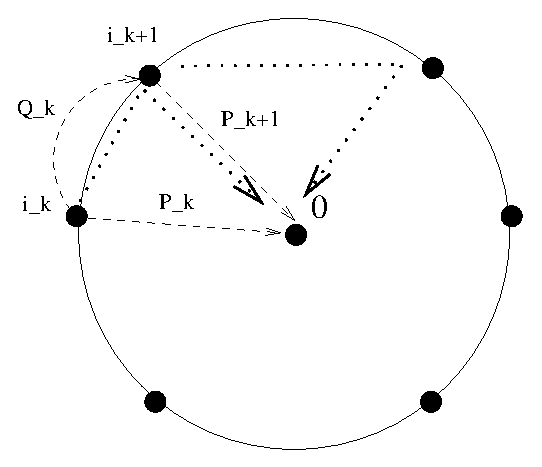
\epsfig{file=policy/figures/dw.eps,width=0.28\textwidth}
\caption[Illustration of an induced path.]{Illustration of an induced 
  path from $v_0$ to $d$, collectively induced by the selection of
  a route to $d$ at every node along the path.  The node $v_i$ may be
  immediately adjacent to $v_0$ (as shown), but it may also be several
  hops away.}
\label{fig:induced_path}
\end{figure}


\begin{defn}[Induced path]\label{defn:ipath}
Let $r_{v_j}(d)$ be the route that node $v_j$ selects en route to $d$
(\ie, it is a mapping $(d \rightarrow v_k)$ for some other $v_k\in G$.
Then, the {\em path induced} by route $r_{v_0}(d): (d \rightarrow v_i)$,
$P_{v_0}(r_{v_0}(d))$, is:
\[
P_{v_0}(r_{v_0}(d)) = \left\{\
\begin{array}{l}
\phi \textrm{ if $v_0$ has no route to $d$ }\\
v_0  \textrm{ if $v_0 \in d$}\\
%(v_0, P_{v_0}(r_{v_0}(v_i)), P_{v_i}(r_{v_i}(d))) \textrm{ otherwise }
(v_0, P_{v_1}(r_{v_1}(d))) \textrm{ otherwise }
\end{array}
\right.
\]
where $v_1$ is defined according to $r_{v_0}(v_i): (d \rightarrow v_1)$;
that is, $v_1$ is the next-hop node in $v_0$'s forwarding table for
destination $v_i$.
\end{defn}

\noindent
Figure~\ref{fig:induced_path} illustrates an induced path and its
constituent subpaths.  The node $v_i$ in the induced path may either be
adjacent to $v_0$ in $G$, or it may be several hops away.  When $v_i$ is
adjacent to $v_0$ in $G$, data traffic can reach $v_i$ from $v_0$ via a direct
IP link.  When $v_i$ is several hops away in $G$, however, $v_0$ must
rely on intermediate nodes to forward traffic to $v_i$.  In this case,
the nodes between $v_0$ and $v_i$ could 
use routes that induce paths that never even traverse $v_i$.
In other words, the path that is described by $(v_0,
P_{v_0}(r_{v_0}(v_i)))$ may traverse an intermediate node whose induced
path to $d$ does not traverse $v_i$.  To precisely
classify the types of paths for which 
this inconsistency does not arise, we define the notion of a consistent
path.

\begin{defn}[Consistent path]
An induced path $P_{v_0}(r_{v_0}(d)) = (v_0, \ldots v_n)$ to $d$ is consistent
if, (1)~for all $1 \leq i \leq n$, $P_{v_i}(r_{v_i}(d)) = (v_i, v_{i+1},
\ldots, v_n)$; (2)~$P_{v_0}(r(v_0(d)))$ contains $v_i$, where
$r_{v_0}(d): d \rightarrow v_i$.
\end{defn}

Consistent paths are an important class of paths because inconsistent
paths can sometimes give rise to forwarding loops.  A {\em forwarding
loop} is a special case of an inconsistent path where some intermediate
node's induced path includes a node that has already appeared on the
path.  

When $v_0$ and $v_i$ are not adjacent, ensuring that all intermediate
nodes select a route $(d\rightarrow v_i)$ will guarantee that an induced
path is consistent.  If an intermediate node selects some route
$(d\rightarrow v_j)$ where $v_i\neq v_j$, then the induced path to $d$
may never traverse $v_i$.  If, on
the other hand, the intermediate node selects a route $(d\rightarrow
v_i)$, then the induced path from that node to $v_i$ will be a subpath
of $P_{v_0}(r_{v_0}(v_i))$, assuming all nodes use the same function to
induce paths (\eg, if the induced path to $v_i$ is based on shortest
paths routing, as in an IGP).


%\subsection{Example: Paths and Routes in Internet Routing}

We now briefly discuss paths and routes in the context of BGP.  To
illustrate the distinction between routes and paths, we examine their
definitions within the context of BGP routing within a single AS.  In
this case, a {\em route} is of the form $(d \rightarrow v_i)$, where $d$
is an IP prefix and $v_i$ is the BGP ``next hop'' (a node that need not
be directly connected at the IP layer).  The {\em path} that traffic
ultimately takes from some node $v_j$ to the destination $d$, for which
$v_j$ has a route $(d \rightarrow v_i)$, depends on how connectivity is
established between $v_j$ and $v_i$.  If $v_j$ and $v_i$ are in two
different ASes, then they are typically directly connected.  If they are
in the same AS, however, it is common for $v_i$ to be the IP address of
an egress (or ``border'') router and for $v_j$ to be several IP hops
away.  The induced path between $v_j$ and $v_i$ may be determined by a
tunnel, by a shortest paths routing protocol, using static routes, etc.

If the induced path between $v_j$ and $v_i$ is not defined by a tunnel,
then the nodes between $v_j$ and $v_i$ will use their own routes for
forwarding data to $d$.  In this case, the induced path to $d$ is
actually determined by ``stitching together'' these constituent induced
paths.  If all nodes between $v_j$ and $v_i$ select routes that indicate
that traffic to $d$ should be sent via $v_i$, then the induced path
between $v_j$ and $v_i$ will be consistent.  Otherwise, the path could
be arbitrary; in fact, it might never traverse $v_i$.

\begin{figure}
\centering
\begin{psfrags}
\psfrag{v1}{{\LARGE $v_1$}}
\psfrag{v2}{{\LARGE $v_2$}}
\psfrag{v3}{{\LARGE $v_3$}}
\psfrag{v4}{{\LARGE $v_4$}}
\psfrag{v5}{{\LARGE $v_5$}}
\psfrag{d}{{\LARGE $d$}}
\psfrag{dr}{{\Large $(d \rightarrow v_5)$}}
%
%\hspace{-0.7in}
\resizebox{0.65\textwidth}{!}{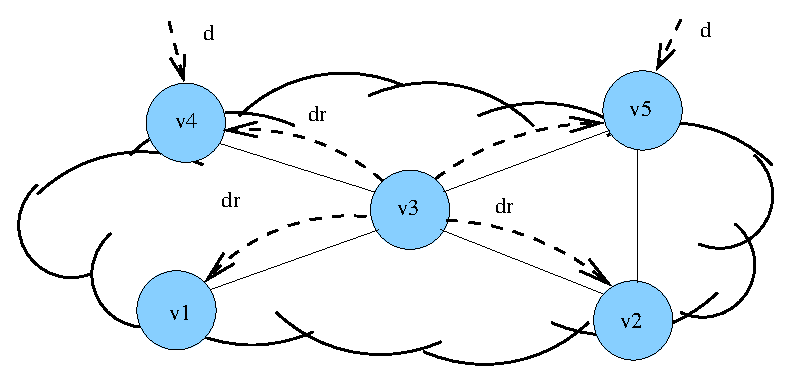
\includegraphics{rlogic/figures/path_route.eps}}
\end{psfrags}
%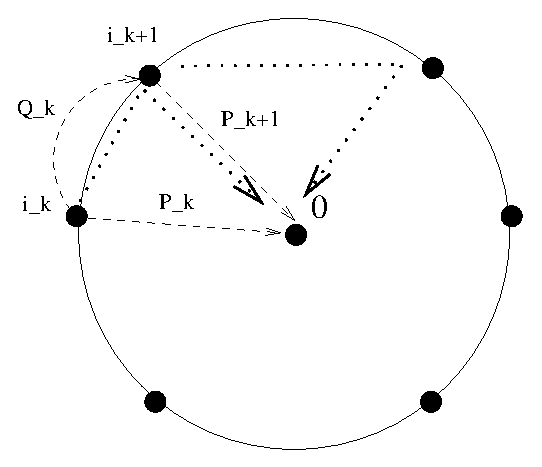
\epsfig{file=policy/figures/dw.eps,width=0.28\textwidth}
\caption[Paths and routes in BGP.]{An example that demonstrates how BGP
  routes induce paths.  Dashed lines are iBGP sessions from route
  reflectors to clients (\ie, $v_3$ is a route reflector, and the rest of
  the routers are its clients); route reflector operation is summarized
  in Section~\ref{sec:dissemination}.  Dashed lines show propagation of
  routes. Solid lines show IGP links; in this example, all links have a
  cost of $1$.  The routes at each node {\em induce} paths over the IGP
  topology. For example, the induced path from $v_2$ to $d$ is $(v_2,
  v_5, ...)$, the induced path from $v_1$ to $d$ is $(v_1, v_3, v_5,
  ...)$, etc.}
\label{fig:path_route}
\end{figure}

Figure~\ref{fig:path_route} shows an example that illustrates this
distinction.  In this example, all routers in the AS are clients of the
route reflector, $v_3$; solid lines show the edges in the IGP graph, and
all edges have a cost of $1$.  Suppose that $v_3$ learns two routes to
$d$ and selects the route that it receives from $v_5$.  In this case,
$v_3$ propagates that {\em route} (\ie, $(d \rightarrow v_5)$) to all of
its clients, as shown.   Using that route, each node ultimately uses a
different {\em path} to the egress router, $v_5$.  For example, $v_1$'s
shortest IGP path to $v_5$ is $v_1,v_3,v_5$, whereas $v_2$'s shortest
path to $v_5$ is $v_2, v_5$.  Even if a node, say $v_1$ selects a BGP
route with the ``next hop'' $v_5$, there is no guarantee that the
resulting {\em induced path} will traverse $v_5$.  If an additional
node, $v_6$, 
had been on the path between $v_1$ and $v_3$, and had instead selected a
route $(d\rightarrow v_4)$, then $v_1$'s path to $d$ through the AS
could have in fact been $v_1, v_6, v_4$.




%For the pursposes of our work, we assume that physical
%links and internal routing is operating correctly.  That is, we assume
%that a path exists between {\em any} source-destination pair where the
%source and destination are in the same AS.

\subsection{Policy}

A noteworthy aspect of Internet routing is that it is {\em policy-based}.
The job of the routing protocol is not to propagate complete
information about the topology, but to only propagate information about
paths that comply with the various economic and policy goals of each AS.
We must therefore qualify paths in the topology according to
those that comply with such these policies and those that do not.

\begin{defn}[Policy]\label{defn:policy}
A {\em policy} is a function $\P(s, v_{i-1},v_{i},v_{i+1},d) \rightarrow
(0,1)$, 
where $s$ is a source, $v_{i-1}$, $v_i$, and $v_{i+1}$ are 
nodes on a path $(v_0, v_1, \ldots, v_n)$, $d$ is a
destination, and $\P$ is defined as follows: 
\[
\P(s,v_{i-1},v_i,v_{i+1},d) = \left\{\
\begin{array}{l}
1\textrm{ if $i=0$ and $v_0$ forwards packets from source $s$ destined
  for $d$}\\ 
1\textrm{ if $0<i<n$ and $v_i$ forwards packets with source $s$ from
  $v_{i-1}$} \\ \textrm{\hspace*{0.2in} destined for $d$ via $v_{i+1}$}\\
1\textrm{ if $i=n$ and $v_n$ forwards packets with source $s$ destined
  for $d$}\\ 
0\textrm{ otherwise }
\end{array}
\right.
\]
\end{defn}

The function $\P(v_{i-1}, v_i, v_{i+1}, d)$ is not expressive enough to
capture all policies, but, as we will see, it is general enough to
capture the policies that are commonly expressed in Internet
routing.  Other routing protocols may require more expressive
policy functions. Our intent here is not to define a policy function
that captures all policies, but rather to allow us to define a
policy-conformant path in the context of Internet routing.

%A value of $0$ indicates that traffic
%should not be allowed to flow on any path from $s$ to $d$; a value of
%$1$ indicates that such a path is permissible.

\begin{defn}[Policy-conformant path]\label{defn:pcp}
A path $(v_0, v_1, v_2, \ldots, v_n)$ is policy-conformant for source $s$
and destination 
$d$ if $\P(s, v_{i-1}, v_i, v_{i+1},d) = 1$ for all $0 \leq i \leq n$.
\end{defn}

\noindent
For simplicity, we assume that paths for which the source,
destination, and all nodes in between the source and destination are in
the same AS are policy-conformant.  
%

\begin{figure}
\centering
\begin{psfrags}
\psfrag{X}{{\Large $X$}}
\psfrag{Y}{{\Large $Y$}}
\psfrag{Z}{{\Large $Z$}}
\psfrag{vx}{$v_X$}
\psfrag{vy1}{$v_i$}
\psfrag{vy2}{$v_j$}
\psfrag{vz}{$v_Z$}
\resizebox{0.9\textwidth}{!}{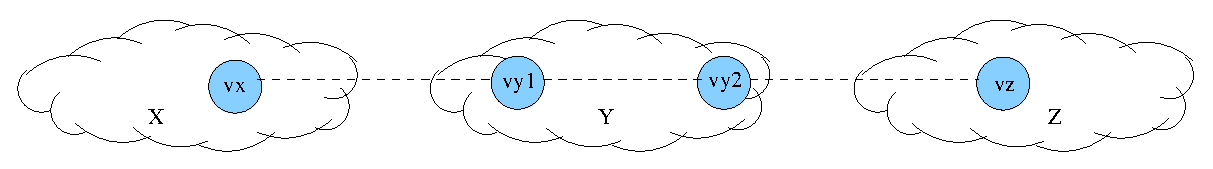
\includegraphics{rlogic/figures/policy_ex.eps}}
\end{psfrags}
\caption[Expressing policy-conformant paths at the AS-level in BGP.]{An example
  illustrating policy-conformant paths at the AS-level in BGP.}
\label{fig:policy_ex}
\end{figure}


%The policy function $\P$ allows an operator to restrict paths that do
%not conform to some policy by expressing $\P(v_{i-1},v_i,v_{i+1},d)$,
%where $v_{i-1}$, $v_i$, and $v_{i+1}$ are nodes in three different ASes.
Although the policy function is defined at the level of nodes, it is in
fact expressive enough to capture many AS-level policies that network
operators commonly want to express.  For example, suppose an operator
wants to express that AS $Y$ should not forward traffic between two other
ASes, $X$ and $Z$, for some destination $d$, as
pictured in Figure~\ref{fig:policy_ex}.  Recall that a path with some
nodes removed still constitutes a path.  As such, it is possible 
to express this policy in terms of the nodes in ASes $X$ and $Z$
along the path.  For example, in Figure~\ref{fig:policy_ex}, the policy can be
expressed as $\P(s, v_X, v_i, v_Z, d) = 0$.  In a more complicated
scenario, if AS $Y$ has multiple nodes that are adjacent to nodes in
ASes $X$ and $Z$, the AS-level policy would be
expressed as an enumeration over node-level policies.



\section{Route Validity}\label{sec:validity_def}

In this section, we motivate and describe {\em route validity}.
Informally, route validity says that any route that the routing protocol
propagates should correspond to a usable path in the topology.  Route
validity concerns the properties of the paths induced by the routes that
the routing protocol propagates.

\begin{defn}[Route validity]\label{defn:rv}
A route for a destination $d$ is valid if, and only if, the path induced
by the route (1)~is consistent, (2)~is policy-conformant for all sources
that use the route, and
(3)~terminates at $d$.  We say that a routing protocol satisfies route
validity if the protocol propagates only valid routes for all
destinations.
\end{defn}


\begin{figure}
\centering
\begin{psfrags}
%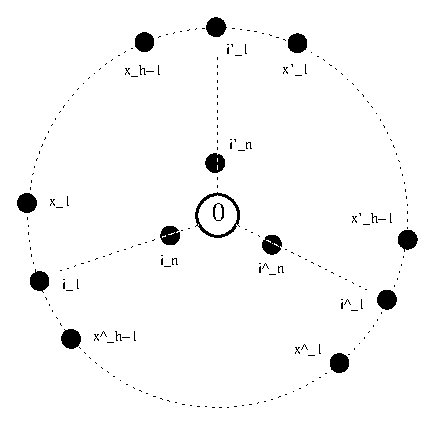
\epsfig{file=policy/figures/lemdr.eps,width=0.25\textwidth}
%
\psfrag{vi}{ $v_i$}
\psfrag{vid}{ $v_n \in d$}
\psfrag{vnd}{ $v_n \in d$}
\psfrag{vi1}{$v_{i-1}$}
\psfrag{v0}{$v_0$}
\psfrag{v1}{$v_1$}
\psfrag{dr}{$(d \rightarrow v_i)$}
\psfrag{d}{$d$}
%
%\hspace{-0.7in}
\resizebox{\textwidth}{!}{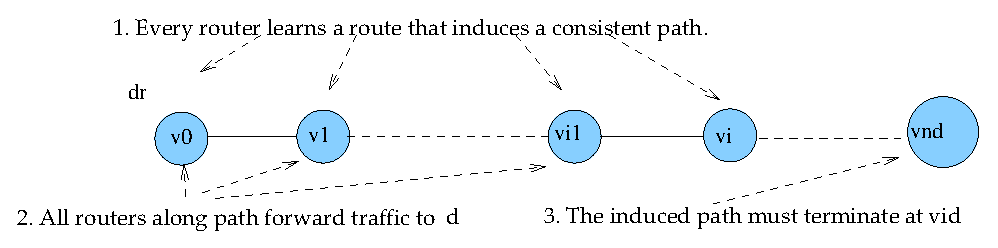
\includegraphics{rlogic/figures/rv_expl.eps}}
\end{psfrags}
%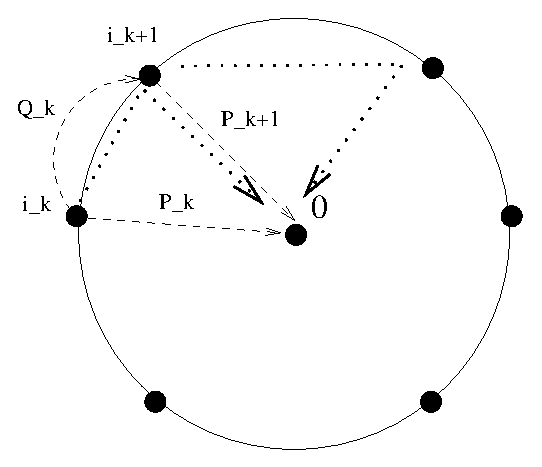
\epsfig{file=policy/figures/dw.eps,width=0.28\textwidth}
\caption[The conditions of route validity.]{The conditions of route
  validity.  A route is valid if it induces a consistent,
  policy-conformant path at every node along the path from $v_0$ to some
  $v_i \in d$.}
\label{fig:rv_expl}
\end{figure}


Figure~\ref{fig:rv_expl} illustrates the conditions of route validity.
The first condition of route validity enforces consistency
along the path between $v_0$ and the node $v_i$ towards which $v_0$
sends traffic en route to $d$.
%If all intermediate nodes
%between $v_0$ and $v_i$ have the same next-hop, $v_i$, then there can be
%no forwarding loops between $v_0$ and $v_i$.  
Furthermore, the induced path from $v_0$ to $v_i$ must be
policy-conformant; that is, every node along the path $(v_0, \ldots, v_i)$
must forward traffic from its predecessor to its next hop en route to
$d$.  Verifying policy conformance is difficult for
paths that traverse multiple ASes, because operators do not explicitly
specify the policy function $\P$.  The final condition says that the
path induced by the route must actually terminate at some node $v_n \in
d$.
%The final condition of route validity says that, once
%traffic reaches the node $v_i$, then that node also has a route to the
%destination that satisfies route validity.


%%%%%%%%%%%%%%%%%%%%%%%%%%%%%%%%%%%%%%%%%%%%%%%%%%%%%%%%%%%%

Because a source $v_0$ and a destination $d$ may be in different ASes,
guaranteeing that BGP satisfies route validity is difficult in practice.
Determining both the induced path to $d$ and determining whether that
path is policy-conformant requires knowledge of the configurations of
multiple ASes.  Fortunately, the properties of route validity (\ie,
consistency and policy-conformance) are composable.

\begin{observation}\label{obs:composable}
Composing a path by concatenating two consistent, policy-conformant
paths results in a new consistent, policy-conformant path.
\end{observation}

This observation implies that if the routing protocols in each AS en
route to a destination induce only consistent and policy-conformant
paths to some destination $d$, then BGP will only induce consistent,
policy-conformant paths for that destination $d$.  For the purposes of
this chapter, we assume that all paths are policy-conformant, because
detecting violations of policy are difficult to verify in practice; we will
return to this issue in Section~\ref{sec:validity}.  We also assume that
all eBGP sessions are point-to-point (\ie, immediately connected at the
IP layer), which is almost always the case in practice: service
providers typically apply policies at AS boundaries, rather than on
paths within an AS.  Finally, we assume that the IGP already satisfies
route validity; detecting route validity faults in internal routing
protocols is beyond the scope of this dissertation.



%% \begin{proof}
%% We must show that, when a route gives rise to a path where any $v_i$ and
%% $v_{i+1}$ are in different ASes, then the path that traverses the two
%% ASes still satisfies the conditions for route validity.  Since the path
%% segment $v_i, v_{i+1}$ is a point-to-point link, then $v_i$ selects the
%% route $(d \rightarrow v_{i+1})$, and the first condition is satisfied.
%% The third condition is satisfied by the inductive assumption.  
%% \end{proof}


Modulo policy-conformance, guaranteeing that BGP satisfies route
validity boils down to ensuring that iBGP always induces consistent
paths within each AS.  Guaranteeing this property is the focus of
the remainder of this section.  We first focus on how to guarantee that
``full mesh'' iBGP configurations (and protocol modifications that
would allow every
router to the complete set of ``best'' eBGP-learned routes) always
induce consistent paths; we 
then derive conditions on iBGP configurations that use route reflection
that guarantee that iBGP only induces consistent paths.

\subsection{Case \#1: Every router learns all ``best'' eBGP routes.}
\label{sec:mesh}

If different routers within an AS receive different sets of candidate
routes for some destination $d$, then the routers along a path from $v_0$
to $v_i$ may not ultimately select the route $(d \rightarrow v_i)$.  It
turns out that the default iBGP configuration, where every eBGP-speaking
router has an iBGP session with every other eBGP-speaking router in the
AS (\ie, a ``full mesh'' iBGP configuration, as described in
Section~\ref{sec:dissemination}, Figure~\ref{fig:fullmesh}) satisfies
route validity.

\begin{figure}
\centering
\begin{psfrags}
%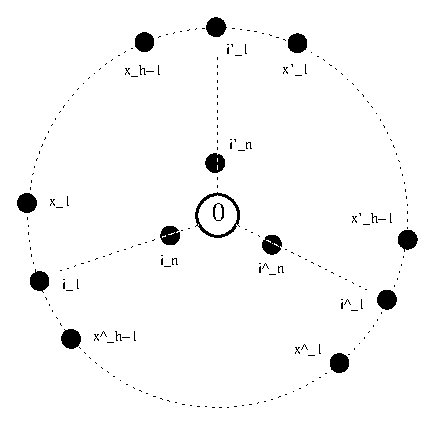
\epsfig{file=policy/figures/lemdr.eps,width=0.25\textwidth}
%
\psfrag{v_i}{{\LARGE $v_i$}}
\psfrag{v_j}{{\LARGE$v_j$}}
\psfrag{a}{{\LARGE $a$}}
\psfrag{b}{{\LARGE$b$}}
\psfrag{s}{{\LARGE$v_0$}}
%
%\hspace{-0.7in}
\resizebox{0.5\textwidth}{!}{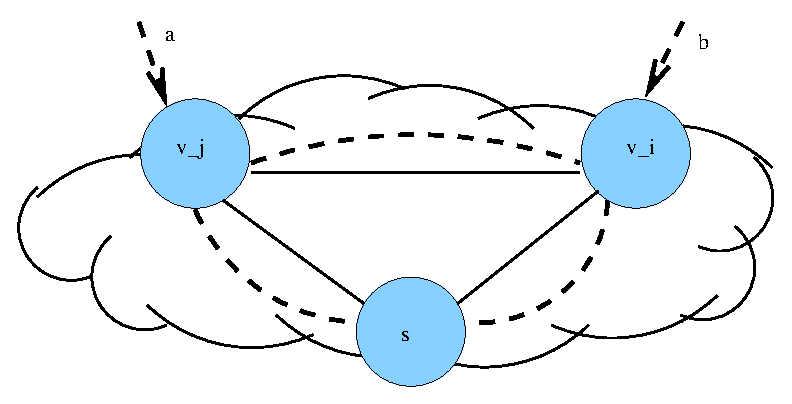
\includegraphics{rlogic/figures/fm_validity.eps}}
\end{psfrags}
%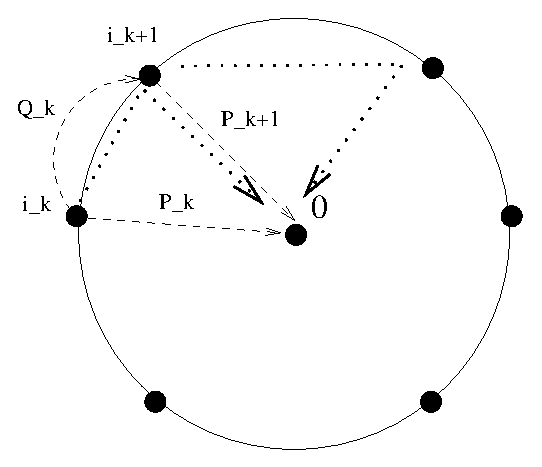
\epsfig{file=policy/figures/dw.eps,width=0.28\textwidth}
\caption[The main idea of the proof of
  Theorem~\ref{th:mesh}]{This figure illustrates the main idea of the proof of
  Theorem~\ref{th:mesh}.  Dashed lines represent iBGP sessions, and
  solid line represent IGP links.  If routes $a$ and $b$ do not have equal
  local preference, AS path length, origin type, or MED, then $v_0$,
  $v_i$, and $v_j$ will all select the same route.  If these attributes
  are equal for both $a$ and $b$, then $v_0$ selects either $a$ or $b$
  depending on whether $v_i$ or $v_j$ has a shorter IGP path.  If $v_j$
  selects route $a$ and $v_i$ selects route $b$, then $v_0$'s shortest IGP
  path to the next hop corresponding to the chosen route must be direct.}
\label{fig:fm_validity}
\end{figure}


\begin{theorem}\label{th:mesh}
If (1)~every router learns the BGP routes selected by the complete set of
eBGP-speaking routers, and
(2)~iBGP-speaking routers do not modify route attributes (\ie, local
preference, origin type, MED, or next hop), then 
all paths induced by iBGP (within the AS) will be consistent.
\end{theorem}

\begin{proof}
If each router eventually learns of the route selected by every
eBGP-speaking router, then there are two cases for any router $v_0$ in
the AS: either (1)~$v_0$ selects a route via a $v_i$ in a neighboring
AS, or (2)~$v_0$ selects a route via $v_i$ in the same AS, where $v_i$ is an
eBGP-speaking router and, hence, in turn selects a route such that
$v_{i+i}$ is in a neighboring AS.  The first case corresponds to a
point-to-point eBGP session; the second case corresponds to an iBGP
session where the route's next hop $v_i$ learned the route via a
point-to-point eBGP session but may be multiple IP hops away.  For the
proof of this theorem, we are only concerned with the latter case; we
rely on Observation~\ref{obs:composable} to ensure that iBGP induces
only consistent paths in neighboring ASes.

%% Route validity holds in the first case, because $v_i$ is in a
%% neighboring AS, and, by assumption, the remainder of the path is
%% consistent.  In the case where $v_i$ is in the same AS, the path $(v_0,
%% \ldots, v_i)$ may include multiple nodes (\ie, routers) in the same AS.
%% We know that $v_i$ selects a route that induces a consistent path
%% because $v_i$ selects a route from a neighboring AS.  

To show that iBGP induces only consistent paths within the AS, we show
that all routers on the path $(v_0, \ldots, v_i)$ select the route $(d
\rightarrow v_i)$, for any $v_i\in G$.  Because all eBGP-speaking
routers have an iBGP session with every other router in the AS, all
routers (and, in particular, all routers along the path $(v_0, \ldots,
v_i)$) learn the same set of ``best'' routes.  All of these routers
would thus select a route with the highest local preference, shortest AS
path length, lowest origin type, and lowest MED.

As a result, we know that all routers along the path $(v_0, \ldots,
v_i)$ select {\em some} iBGP learned route with the shortest IGP path
among candidate iBGP routes.  Suppose that some router on this path, say
$v_j$, selects a route other than $(d \rightarrow v_i)$, say $(d
\rightarrow v_k)$, because $(v_j, \ldots, v_k)$ has a shorter path cost
than $(v_j, \ldots, v_i)$.  Then, the nodes in $(v_0, \ldots, v_k)$ {\em
also} have a shorter IGP path cost than $(v_0, \ldots, v_i)$ and, hence,
all nodes in $(v_0, \ldots, v_{k-1})$ would also select $(d \rightarrow
v_k)$.
\end{proof}

A full mesh iBGP configuration can guarantee the first condition of
Theorem~\ref{th:mesh}.  Another approach to ensuring that every router
learns the set of routes selected by the complete set of eBGP-speaking
routers is to alter how route reflectors readvertise routes to their
clients.  By a similar argument as in the proof of
Theorem~\ref{th:mesh}, such a modification would cause iBGP to induce
only consistent paths.  Such a configuration not only guarantees
consistent paths, but it also prevents certain types of persistent route
oscillation (a pathology we examine in more detail in
Section~\ref{sec:safety_def})~\cite{Basu2002}. Unfortunately,
implementing such a configuration in practice requires modifying the
large deployed base of BGP routers.  Alternatively, an architecture such
as either the Routing Control Platform
(RCP)~\cite{caesar2004,feamster:fdna2004} or the recent proposal for
more versatile route reflectors~\cite{id-versatile-rr} could implement
this type of iBGP configuration.


%% \begin{defn}[RR-Reflect-All]
%% A route reflector configuration for an AS is {\em RR-Reflect-All} if all
%% route reflectors for that AS advertise all routes to a particular
%% destination (as opposed to simply the best route), and route reflectors
%% readvertise all routes with each other (\ie, path visibility is
%% satisfied among router reflectors).
%% \end{defn}

%% \begin{theorem}\label{th:rr_reflect}
%% If the route reflectors in an AS are configured according to {\em
%% RR-Reflect-All}, then all paths induced by iBGP are consistent.
%% \end{theorem}

%% \begin{proof}

%% In an {\em RR-Reflect-All} iBGP configuration, all routers ultimately
%% receive all routes to a destination $d$.  There are two cases:
%% (1)~there exists only one route that is better according to the first
%% four steps of the BGP route selection process (local preference, AS path
%% length, 
%% origin type, MED); (2)~there exists more than one route to $d$, and ties
%% between multiple candidate routes are broken after the first four steps.
%% In the first case, all routers will select that single route with common
%% next hop, so route validity is satisfied because every router selects
%% the same next hop.  In the second case, either a router $v_0$ selects a
%% route via its own eBGP session, if one exists (in which case route
%% validity is trivially satisfied again) or it selects a route that
%% traverses other routers in the same AS to reach the next hop $v_i$.
%% Because every router receives all routes to a destination, if some
%% router on the shortest path between $v_0$ and $v_i$ selects a route with a
%% next-hop other than $v_i$, then $v_0$ would have also selected the route
%% with that next hop, by the same argument in Theorem~\ref{th:mesh}.
%% \end{proof}





\subsection{Case \#2: Each router learns only some ``best'' eBGP routes}

If full mesh iBGP were the only intra-AS BGP configuration,
guaranteeing that iBGP satisfied route validity would be easy.
Unfortunately, as discussed in Section~\ref{sec:dissemination}, this
technique does not scale to large ASes because it requires $O(|R|^2)$
iBGP sessions, where $|R|$ is the number of routers in the AS.  Large
ASes typically use a 
technique called route 
reflection, where a single route reflector selects a route on behalf of
its client routers.


\begin{figure}
\begin{center}
\begin{psfrags}
\psfrag{RR1}{{\LARGE $RR_1$}}
\psfrag{RR2}{{\LARGE $RR_2$}}
\psfrag{C1}{{\LARGE $C_1$}}
\psfrag{C2}{{\LARGE $C_2$}}
\psfrag{d}{{\LARGE $d$}}
%\centering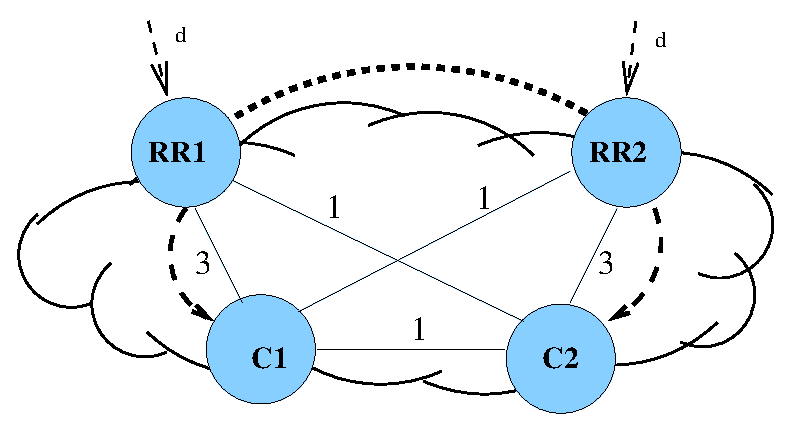
\epsfig{file=rlogic/figures/dube.eps,width=0.7\textwidth}
\resizebox{0.5\textwidth}{!}{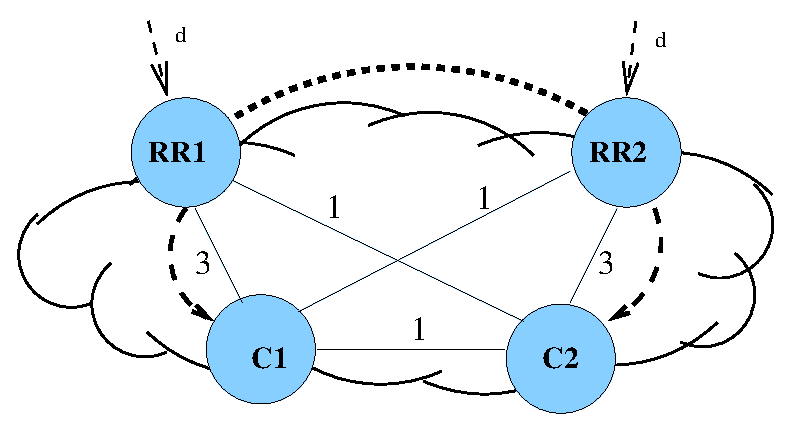
\includegraphics{rlogic/figures/dube.eps}}
\end{psfrags}
\end{center}
\caption[The interaction of IGP and route reflection may cause
  forwarding loops.]{The interaction of IGP and route reflection in iBGP
  may cause route validity violations resulting in forwarding
  loops~\cite{Dube99}. 
  Note that this topology satisfies path visibility but not route
  validity.  Dashed lines represent iBGP sessions; a directed edge
  indicates an iBGP sessions from a route reflector to its client.}
\label{fig:dube}
\end{figure}


Guaranteeing route validity in an iBGP topology with route reflectors is
not easy.  Previous work has observed that the interactions between the
IGP topology and an iBGP topology with route reflectors can give rise to route
validity violations~\cite{Dube99}.  Figure~\ref{fig:dube} shows one such
example.  Route reflectors $RR_1$ and $RR_2$ both receive a route to
destination $d$ and have clients $C_1$ and $C_2$ respectively.  Hence,
$C_1$ may receive and select the route $(d \rightarrow RR_1)$, and $C_2$
may receive and select the route $(d \rightarrow RR_2)$.  If the
shortest IGP path (\ie, the induced path) between $A$ and $RR_1$ is via
$B$, and the shortest 
IGP path between $B$ and $RR_2$ is via $A$, then traffic en route to $d$
that traverses either router $A$ or $B$ will be caught in a persistent
{\em forwarding loop}: that is, traffic destined for $d$ will never
reach $d$ but instead will repeatedly visit a cycle of two or
more nodes.  A forwarding loop is simply a special case of a route
validity violation.

Our goal is to detect whether a configuration of route reflectors and
clients induces only consistent paths with a simple algorithm that
examines only the static iBGP and IGP topologies.  One such sufficient
condition that guarantees this property requires that the iBGP topology
be {\em RR-IGP-Consistent}, defined as follows:

\begin{defn}[RR-IGP-Consistent]\label{defn:igp-consistent}
A route reflector configuration is {\em RR-IGP-Consistent} if, for all
nodes, every shortest IGP path between that node and its possible egress
nodes (\ie, the set of eBGP-speaking routers) traverses that node's
route reflector before any other node's route reflector and the egress
node's route reflector before the egress node itself.
\end{defn}
In previous work, Dube suggested placing route
reflectors on the shortest IGP path to their clients~\cite{Dube99}.  We
now prove that this condition guarantees that the iBGP configuration
will only induce consistent paths.  

\begin{theorem}\label{th:rr_safe}
If an iBGP configuration is {\em RR-IGP-Consistent}, then
all paths induced by iBGP are consistent.
\end{theorem}

\begin{proof}
Suppose not.  Then, there must exist a
destination $d$ and a path $P = (v_0, \ldots, v_n)$ for which some node $v_j$
between $v_0$ and $v_n$ selects a route $(d \rightarrow v_i)$, where $i
\neq n$.  There are two cases: (1)~$v_j$ is on the path from $v_0$ to the
route reflector of $v_0$; and (2)~$v_j$ is on the path from the route
reflector of $v_0$ to $v_n$.  

In the first case, if $v_0$ and $v_j$ select different next hops then, by
definition, they must be clients of different route reflectors.
By definition, then, the iBGP topology is not {\em RR-IGP-Consistent}.
%Then,
%it must be the case that either $v_0$'s path to $v_n$ goes through $v_j$'s
%route reflector before its own route reflector, or $v_j$'s path to $v_n$
%goes through $v_0$'s route reflector before its own route reflector.
%Either case implies that {\em RR-IGP-Consistent} is not satisfied.
The second case reduces to a similar argument as in
Theorem~\ref{th:mesh}: if $v_j$ selects a route with a next hop other
than $v_n$, then the route reflector of $v_0$ would have also learned that
route and selected it (otherwise, $v_j$ would not have been on the route
reflector's shortest path to $v_n$, by the same argument as in
Theorem~\ref{th:mesh}).
\end{proof}

Although this result is a helpful sufficient condition, it does not
guarantee that route validity will be satisfied when arbitrary links
fail, thus causing shortest IGP paths to change.  Designing an {\em
RR-IGP-Consistent} iBGP topology that is robust to link failures is a
difficult task.  Recent work has proposed using graph separators as a
way of efficiently placing route reflectors in an iBGP topology 
to guarantee that route validity is satisfied~\cite{Vutukuru2005}.  


%%%%%%%%%%%%%%%%%%%%%%%%%%%%%%%%%%%%%%%%%%%%%%%%%%%%%%%%%%%%

\section{Path Visibility}\label{sec:visibility_def}

Path visibility says that if there exists one or more policy-conformant
paths between two 
nodes, then the routing protocol should propagate routes that 
induce at least one of those paths.  Path visibility is an important
property for a number of reasons.  First, if a routing protocol
satisfies this property, then every node is guaranteed to have the
necessary information to reach all other nodes.
%Essentially, it states that the routing protocol is propagating
%enough information to allow any node to reach any other node for which
%it has a path in the underlying topology.  
%Second, as is evident from the
%theorems of Section~\ref{sec:validity_def}, an iBGP configuration must
%satisfy path visibility in order to satisfy route validity.

\begin{defn}[Path visibility]\label{defn:pv}
A routing protocol satisfies {\em path visibility} if, for all $v_0\in
V$ and for all destinations $d$, the existence of a policy-conformant
path $P = (v_0, \ldots, v_n)$ implies that $v_0$ learns a valid route
$(d \rightarrow v_j)$ for some $0 \leq j \leq n$.
\end{defn}

Path visibility states that if there is a policy-conformant
path from $v_0$ to $d$, then $v_0$ should learn {\em at least one} valid
route to $d$.  Note that the definition does not require $v_0$ to learn
all routes to $d$, nor does it require that $v_0$ learn the ``best''
route to $d$ by any metric.  Path visibility also does not require that
the route that $v_0$ learns correspond to the actual path that traffic
takes from $v_0$ to $d$.
%Although these might all be
%desirable properties, path visibility only requires the minimal
%conditions for correctness: as long as there is a policy-conformant path
%from $v_0$ to $d$, the routing protocol should propagate information that
%allows $v_0$ to send traffic to $d$.

By definition, path visibility violations result when some router fails
to propagate usable routes. These failures in route propagation 
range from the mundane (\eg, misconfigured filters that fail to
install or advertise routes for a policy-conformant path) to the subtle
(\eg, errors in iBGP configuration).

\begin{figure}
\begin{center}
\begin{psfrags}
\psfrag{R1}{{\LARGE $RR_1$}}
\psfrag{R2}{{\LARGE $RR_2$}}
\psfrag{R3}{{\LARGE $RR_3$}}
\psfrag{X}{{\LARGE $C_1$}}
\psfrag{Y}{{\LARGE $C_2$}}
\psfrag{Z}{{\LARGE $C_3$}}
\resizebox{0.6\textwidth}{!}{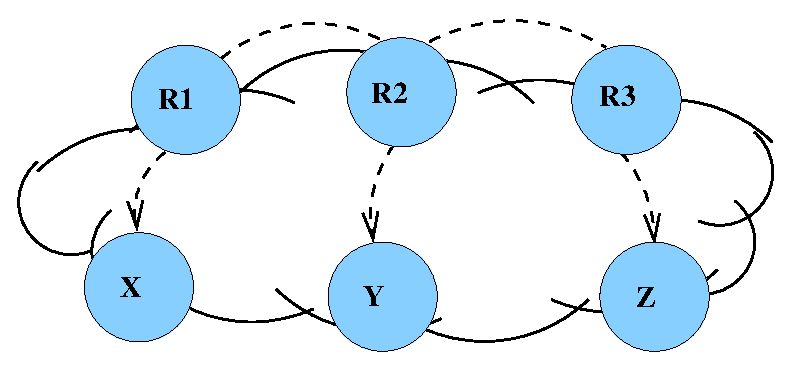
\includegraphics{rlogic/figures/ibgp_rr_pv.eps}}
\end{psfrags}
\end{center}
\caption[A simple iBGP topology that violates path visibility.]{A simple
  iBGP topology that violates path visibility.  Routes learned via eBGP
  at $RR_1$ or $C_1$ will not be propagated to $RR_3$ or $C_3$ (and vice
  versa).}
\label{fig:rl:ibgp_rr}
\end{figure}


Because of the way iBGP readvertises routes, an arbitrary iBGP
configuration is not guaranteed to satisfy path visibility.  In fact,
even the very 
simple iBGP topology in Figure~\ref{fig:rl:ibgp_rr} does not satisfy
path visibility: if the route reflector $RR_1$ (or its client, $C_1$)
receives a route for some destination via an eBGP session, then neither
$RR_3$ nor $C_3$ will receive a route to the destination, and vice
versa.  


Path visibility is important because it ensures that, if the network
remains connected at lower layers, the routing protocol does not create
any new network partitions.  Path visibility also reduces the likelihood of
suboptimal routing.  For example, in Figure~\ref{fig:rl:ibgp_rr}, even if
all clients learned {\em some} route to the destination via eBGP, the
clients would not be guaranteed to discover the {\em best} route to the
destination (\eg, if a client of the route reflector on the far left
learned a route with a shorter AS path, neither the route reflector on
the far right nor its clients would learn it).  As such, it is important
that an AS's iBGP configuration satisfy path visibility.  In the
remainder of this section, we derive the constraints on the iBGP
configuration that must be satisfied to guarantee path visibility.  We
first consider iBGP topologies that do not employ route reflection.


\begin{theorem}\label{th:mesh_visibility}
For an iBGP topology without route reflectors,
satisfying path visibility requires a full mesh iBGP configuration.
%that every router have an iBGP
%session with every router that may learn a route via eBGP (\ie, all
%routers are ``fully meshed'' with the eBGP-speaking routers).
\end{theorem}

\begin{proof}
Consider a router $v_i$, which learns a route $r$ for some destination $d$ via
eBGP, and a router $v_0$ within the same AS that does not have an iBGP
session to $v_i$.  Then, $v_i$ will readvertise $r$ to the routers to which
it has iBGP sessions, but none of those routers will advertise the route
to $v_0$, because they all learned the route via iBGP.
\end{proof}

%% Note that an iBGP configuration without route reflectors does {\em not}
%% require every router to have an iBGP session with every other router (as
%% is commonly stated): the routers that do not receive any routes to a
%% destination via eBGP need not have iBGP sessions with each other.


In large networks, a route reflector may itself be a client
of another route reflector.  Any router may also have ``normal'' (\ie,
peer) iBGP sessions with other routers.  We use the set of
reflector-client relationships between routers in an AS to define a
graph $\I$, where each router is a node and each session is either a
directed or undirected edge: a client-reflector session is a directed
edge from client to reflector, and peer iBGP sessions are undirected
edges. We say that $\I$ is {\em acyclic} if $\I$ has no sequence of
directed and undirected edges that form a cycle.  In typical iBGP
hierarchy designs, $\I$ is acyclic (previous work states that $\I$ should
be acyclic to prevent protocol oscillations~\cite{Griffin2000}---and it
is a good design decision anyway---although
we will see in Section~\ref{sec:safety_def} that this constraint is
unnecessary).  We now define the topological constraints on $\I$ to
guarantee path visibility.


\begin{theorem}\label{thm:vis}
Suppose that the graph defined by an AS's iBGP relationships, $\I$, is
acyclic.  Then, $\I$ does not have a signaling partition if, and only
if, the eBGP-speaking routers that are not route reflector clients form
a clique. 
\end{theorem}

\begin{figure}
\centering
\begin{psfrags}
\psfrag{c0}{}
\psfrag{c1}{}
\psfrag{c2}{}
\psfrag{RR0}{$RR_0$}
\psfrag{RR1}{$RR_1$}
\psfrag{RR2}{$RR_2$}
\resizebox{0.5\linewidth}{!}{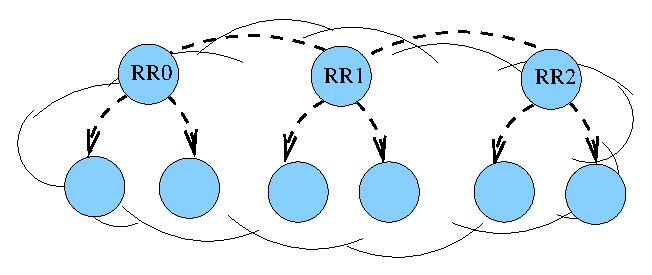
\includegraphics{rlogic/figures/path_vis_ibgp.eps}}
\end{psfrags}
\caption[The main idea of the proof of
  Theorem~\ref{thm:vis}.]{Illustrating the main idea of the proof of
  Theorem~\ref{thm:vis}.}
\label{fig:path_vis_ibgp}
\end{figure}

\begin{proof}
Call the set of routers that are not reflector clients the ``top layer''
of $\I$.  If the top layer is not a clique, then there are two routers
with no iBGP session between them, such that no route learned via eBGP
at $RR_i$ will ever be disseminated to $RR_j$, since no router
readvertises an iBGP-learned route (\eg, $RR_0$ and $RR_2$ in
Figure~\ref{fig:path_vis_ibgp}), and vice versa.  Furthermore, no route that
is learned via eBGP at any of $RR_i$'s clients will be disseminated to
$RR_j$ or $RR_j$'s clients, and vice versa.

Conversely, suppose the top layer is a clique. Observe that if a route
reflector has a route to the destination, then all of its clients have a
route as well.  Thus, if every router in the top layer has a route, all
routers in the AS will have a route.  If any router in the top layer
learns a route through eBGP, then all the top layer routers will hear of
the route (because the top layer is a clique).  Alternatively, if no
router at the top layer hears an eBGP-learned route, but some other
router in the AS does, then that route propagates up a chain of route
reflectors (each client sends it to its reflector, and the reflector
sends it on all its iBGP sessions) to the top layer, from there to all
the other top-layer routers, and from there to the other routers in the
AS.
\end{proof}

The results in this section suggest that path visibility can be
guaranteed by checking relatively simple constraints on the iBGP
topology, which can be determined by analyzing the static configuration
files alone.  Although, in the long term, architectural changes could be
made to guarantee that no configuration ever violates path
visibility~\cite{id-versatile-rr, caesar2004, feamster:fdna2004},
relatively simple checks against routing configuration can guarantee
path visibility today (as we will see in Chapter~\ref{chap:rcc}). 



\section{Safety}\label{sec:safety_def}

%In this section, we discuss properties related to improving
%predictability in Internet routing: {\em safety} and {\em determinism}.
Violations of safety can cause the routing protocol
to continually send routing updates that do not reflect changes in the
underlying topology.  We provide an informal definition of
safety and defer a formal definition to Chapter~\ref{chap:policy}
(Definition~\ref{def:safety}).

\begin{defn}[Safety]
A routing protocol satisfies {\em safety} if and only if, given no
changes to available paths after time $t_0$, then, at some finite time
$t_s > t_0$, each node $v\in G$ selects some route $r$ and does not
select a route $r'\neq r$ for any $t > t_s$.
\end{defn}

Safety is an important property because it guarantees that changes in
{\em routes} (\ie, routing update messages) correspond directly to
changes in available {\em paths}.  This invariant is important for
several reasons.  First, if the routing protocol causes routers to
change routes unnecessarily (\ie, when the paths are in fact stable),
the protocol itself may cause performance degradations, such as lost or
reordered packets.  Second, if routing changes do not correspond to
changes in the actual topology, then debugging the cause of an
oscillation becomes more difficult, because an operator cannot determine
whether routing changes reflect problems with infrastructure (\eg, flaky
or failing equipment) or the routing protocol itself.

Safety problems arise for two reasons:
\begin{enumerate}
\itemsep=-1pt
\item Conflicting route selections within the same AS, caused by
  interactions between BGP route attributes and the IGP (iBGP safety).
\item Conflicting rankings, caused by conflicting policies between
  ASes (eBGP safety).
\end{enumerate}
In both cases, guaranteeing safety is hard.  The
rest of this section focuses on the constraints for guaranteeing safety
in iBGP.  Guaranteeing that eBGP satisfies safety requires either 
knowing the rankings of ASes across the {\em global} Internet (not
a realistic requirement, because ASes typically insist on keeping their
rankings private) or placing restrictions on how each AS can specify
rankings and filters.  This problem is the focus of
Chapter~\ref{chap:policy}.

Safety violations in iBGP occur because BGP's route selection process
(as described in Table~\ref{tab:background:decision},
Section~\ref{sec:bg:route_selection}) does 
not satisfy {\em determinism}.  Determinism essentially says that the
route each router ultimately selects should not depend on either 
(1)~the presence or absence of routes
that would not be selected in the first place or
(2)~the
order in which messages arrive.  We formally define
determinism and explain why guaranteeing this property is difficult in
practice.
\begin{defn}[Selection function]
A selection function at router $r$, $\lambda_r$, takes as input a set of
routes $R_d = \{r_1, \ldots, r_n\}$ for some destination $d$ and produces
a single route $r_i \in R_d$.  The route $r_i$ is often called the
router's ``best route'' to $d$.
\end{defn}

\begin{defn}[Determinism]\label{def:determinism}
A routing protocol satisfies {\em determinism} for destination $d$ if,
for all routers $r$, if $r$ has a set of routes $R_d$ to $d$,
$\lambda_r(R_d)$ satisfies the following two properties:
\begin{enumerate}
\itemsep=-1pt
\item $\lambda_r(R_d) = \lambda_r(R'_d)$, where $R'_d$ is any subset of
  $R_d$ that contains $\lambda_r(R_d)$, and
\item $\lambda_r(R_d)$ does not depend on the order in which the routes
  in $R_d$ arrived at router $r$.
\end{enumerate}
Determinism depends only on the
selection function, $\lambda_r$, for all routers $r$.  Thus, we may also
discuss a single selection function, $\lambda_r$, in terms of whether it
satisfies determinism.
%% Let $\Sigma(R_d) = \{\sigma_1(R_d), \ldots, \sigma_{n!}(R_d)\}$ as
%% the set of all permutations of $R_d$ (\ie, the set of all possible
%% arrival orders for the candidate routes to $r_d$.
%% %
%% Let $T(R_d) = \{t_1(R_d), \ldots, t_{2^n}(R_d)\}$ be the set of all
%% subsets of $R_d$. 
%% %
%% Then, determinism is satisfied if and only if, for all $r_i \in
%% R_d$, $\lambda_r(R_d) = r_i \Rightarrow (r_i \in t_i(R_d) \Rightarrow
%% \lambda_r(\sigma_i(t_i(R_d))) = r_i)$, for all $\sigma_i \in \Sigma(R_d),
%% t_i \in T(R_d)$.
\end{defn}

%% In other words, if a router $r$ selects a certain route as its best
%% route from a set of candidate routes, then it should {\em always} select
%% that route if other routes are removed from that candidate set, and it
%% should always select that route regardless of the order in which
%% those routes arrive at router $r$.
Determinism is important for predictability; moreover, as the following
observation shows, violations of determinism can induce safety
violations, even when the selection function of only one router violates
determinism.


\begin{figure}
\centering
\begin{psfrags}
\psfrag{R1}{{\Large $R_1$}}
\psfrag{R2}{{\Large $R_2$}}
\psfrag{1}{$1$}
\psfrag{2}{$2$}
\psfrag{A}{$A$}
\psfrag{B}{$B$}
\psfrag{C}{$C$}
\psfrag{r1}{$\lambda_{R_1}(\{A,B\}) = A$; $\lambda_{R_1}(\{A,C\}) = C$}
\psfrag{r2}{$\lambda_{R_2}(\{A,B, C\}) = C$;  $\lambda_{R_2}(\{B,C\}) = B$}
\psfrag{A/P}{$A/\phi$}
\psfrag{B/C}{$B/C$}
%
\hspace{-0.4in}
\resizebox{0.7\textwidth}{!}{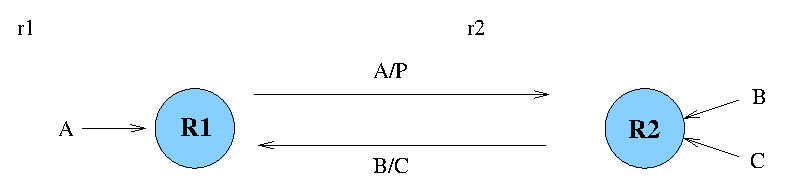
\includegraphics{rlogic/figures/det_a.eps}}
\end{psfrags}
%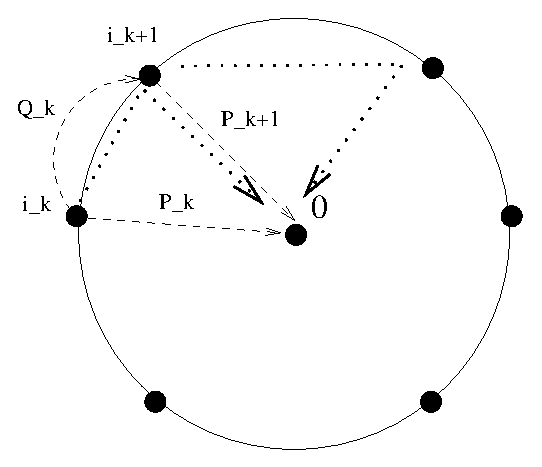
\epsfig{file=policy/figures/dw.eps,width=0.28\textwidth}
\caption[How determinism violations can cause safety
  violations.]{$\lambda_{R_2}$ does not satisfy determinism.  This violation
  can causes a safety violation.}
\label{fig:determinism}
\end{figure}


\begin{figure}
\centering
\begin{psfrags}
\psfrag{R1}{{\Large $R_1$}}
\psfrag{R2}{{\Large $R_2$}}
\psfrag{R3}{{\Large $R_3$}}
\psfrag{1}{$1$}
\psfrag{2}{$2$}
\psfrag{3}{$3$}
\psfrag{A}{$A$}
\psfrag{B}{$B$}
\psfrag{C}{$C$}
\psfrag{r1}{$\lambda_{R_1}(\{A,C\}) = C$;  $\lambda_{R_1}(\{A,B\}) = A$}
\psfrag{r2}{$\lambda_{R_2}(\{A,B, C\}) = C$;  $\lambda_{R_2}(\{B,C\}) = B$}
\psfrag{A/P}{$A/\phi$}
\psfrag{B/C}{$B/C$}
%
\hspace{-1.5in}
\resizebox{0.7\textwidth}{!}{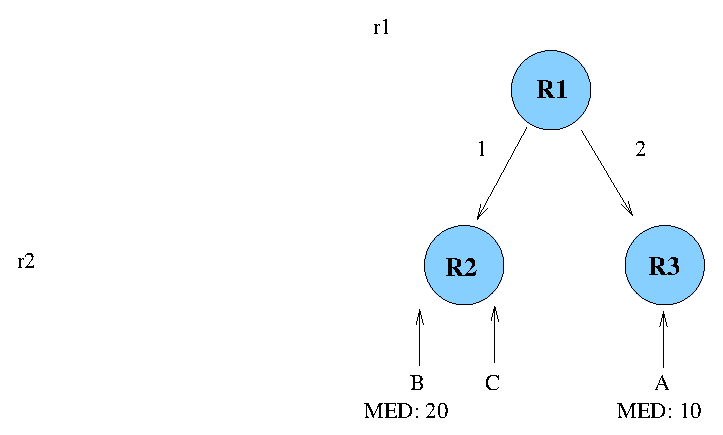
\includegraphics{rlogic/figures/det_b.eps}}
\end{psfrags}
%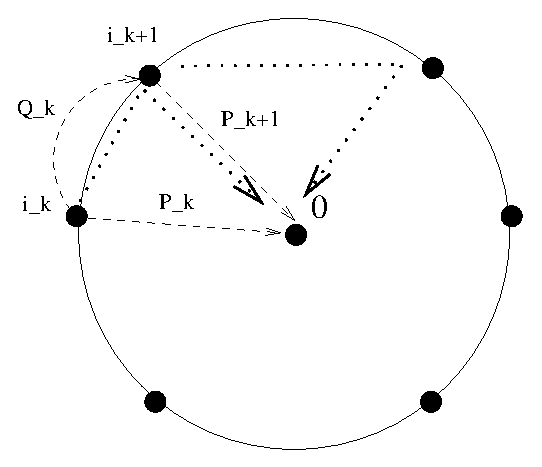
\epsfig{file=policy/figures/dw.eps,width=0.28\textwidth}
\caption[Instantiation of Figure~\ref{fig:determinism} in a BGP
  configuration.]{Instantiation of Figure~\ref{fig:determinism} in a BGP
  configuration.  Router $1$ is a route reflector with two clients, $R_2$
  and $R_3$.  Costs on edges are IGP path costs.  Router $R_2$ prefers route
  $B$ over route $C$ due to a tiebreak.}
\label{fig:determinism_bgp}
\end{figure}

\begin{observation}
If the selection function of even one router, $\lambda_r$, violates
determinism, then the routing protocol may also violate safety.
\end{observation}

\noindent
The following example illustrates this point.

\begin{example}\label{ex:med_det}
Consider Figure~\ref{fig:determinism}.  Router $R_1$ selects route $A$
given the choices $\{A, B\}$ and selects route $C$ given choices
$\{A,C\}$. This selection function satisfies determinism.
On the other hand, router $R_2$'s selection function violates determinism:
$\lambda_{R_2}(\{A,B,C\}) = C$, but $\lambda_{R_2}(\{B,C\}) = B$.  The
interaction of the two selection functions creates the following
oscillation: 
\begin{enumerate}
\itemsep=-1pt
\item Router $R_1$ receives only route $A$, selects it, and
  advertises this route to router $R_2$.
\item Router $R_2$ has received $\{A,B,C\}$, selects
  route $C$, and advertises it to router $R_1$.
\item Router $R_1$ has received $\{A,C\}$, selects
  route $C$, and sends a withdrawal ($\phi$) for route $A$ to router
  $R_2$. 
\item Router $R_2$ selects $B$ from the set $\{B,C\}$ and advertises it to
  router $R_1$, implicitly withdrawing route $C$. 
\item Router $R_1$ now has to select a route from the set $\{A,B\}$, selects
  route $A$, and advertises it to router $R_2$.
\end{enumerate}
This process repeats forever, violating safety.
\end{example}

\subsection{Determinism Violations in BGP: The MED Attribute}

It turns out that the above scenario can occur in BGP, because the MED
attribute causes each router's selection function to violate
determinism.  The addition of a third router, as shown in
Figure~\ref{fig:determinism_bgp}, gives rise to the oscillation from the
previous example.  In this case, router $R_1$ is a route reflector for
two clients: routers $R_2$ and $R_3$, with IGP costs as shown.  Routes
$A$ and $B$ are advertised by the same AS, and route $A$ has a lower MED
value (and, hence, is preferred to $B$).  In this setup, the selection
functions are exactly as described 
in the from Figure~\ref{fig:determinism}: when router $R_2$ learns $\{A,B,C\}$,
route $B$ is eliminated due to MED, and route $C$ is selected because it
is an eBGP-learned route.  When router $R_2$ learns only $\{B,C\}$, on
the other hand, it prefers route $B$ over route $C$ due to the router ID
tiebreak.  Similarly, router $R_1$ prefers route $C$ over route $A$ due
to IGP, but router $A$ over router $B$ due to MED.  The routing system
in this example oscillates in the same fashion as the one shown in
Figure~\ref{fig:determinism}. 

As the above example shows, the interaction between the MED attribute
and route reflection can cause BGP to violate safety.  Note that this
example satisfies the guidelines that were specifically proposed to
avoid these types of oscillations~\cite{rfc3345}.  Even though not all
safety violations are caused by violations of determinism, eliminating
BGP's determinism problem can eliminate all oscillations that do not
involve cyclic preferences over routes caused by setting the local
preference attribute.  Specifically, by making the MED attribute
comparable across {\em all} routes, rather than just those from the same
AS, each router's selection function can be made to satisfy determinism.
We now formally show this result.

\begin{lemma}\label{lem:det_med}
If a router's selection function compares the MED attribute across all
routes to a destination (rather than just across those from the same
neighboring AS), then its selection function satisfies determinism.
\end{lemma}

\begin{proof}
We must show that if the router's selection function compares the MED
attribute across all routes to a destination then: (1)~the route it
selects does not change when any route is removed from that set; and
(2)~the route it selects does not depend on the order in which the
router receives them.

When a router compares the MED attribute across all routes to a
destination, then all routes to a destination can be totally ordered.
Specifically, all routes can be sorted by local preference.  Each set of
routes with equal local preference can be sorted from shortest AS path
length to longest, and so forth.  Thus, the set of routes to a
destination can 
be totally ordered, and removing a route from that set that is not the
most preferred in the total ordering will not change the most preferred
route, since that route must have had a lower local preference, longer
AS path length, higher origin type, lower MED, etc.  

We must also show that the route a router $r$ selects, $\lambda_r(R_d)$,
does not depend on the order that $r$ receives the routes in $R_d$.
%Define two message arrival orders, $\sigma_i(R_d)$ and $\sigma_j(R_d)$,
%and suppose that $\lambda_r(\sigma_i(R_d)) = \rho_i \in R_d$, but
%$\lambda_r(\sigma_j(R_d)) = \rho_j \in R_d$, where $\rho_i \neq \rho_j$.
We know that the routes in $R_d$ are totally ordered, which means that
there is a preference relation between any two routes $\rho_i$ and
$\rho_j$ that is consistent for {\em any} subset of $R_d$ that contains
both $\rho_i$ and $\rho_j$.  We also know that $\lambda_r(R_d)$ will
ultimately select the route that is most preferred in that total
ordering.  Suppose that most preferred route is $\rho_i$.  When $\rho_i$
arrives, $r$ will select $\rho_i$ and continue to select it even after
other routes arrive.  Thus, if $\rho_j$ arrives before $\rho_i$, then
the router will not continue to select $\rho_j$ after $\rho_i$ arrives,
since $\rho_i$ is strictly better than $\rho_j$ in the total ordering.
Similarly, if $\rho_j$ arrives after $\rho_i$, then $r$ will continue to
select $\rho_i$, since it is better than $\rho_j$ in the total ordering.
\end{proof}

We explore how comparing the MED attribute across all routes affects
protocol operation, as well as how this might be done in practice, in
Section~\ref{sec:sandbox:med_disc}.  In short, the primary benefit of
making the route selection function deterministic is that a set of
routers {\em 
within a single AS} may violate safety if determinism is not
satisfied.  Although determinism prevents safety violations such as
those shown in Figures~\ref{fig:determinism}
and~\ref{fig:determinism_bgp}, it does not prevent {\em all} violations
of safety.  For that, we require a stronger notion of determinism, which
we call {\em egress determinism}.


\subsection{Egress Determinism Violations in BGP: Route Reflection}

Even if determinism is satisfied, an AS's iBGP topology can still cause
a routing protocol to violate
safety.  In particular, we can construct an oscillation that
involves the interaction between an AS's route reflector topology and
its IGP topology.  To better understand this interaction, we first
define the notion of {\em egress determinism}.  Egress determinism is a
stronger condition than determinism, as shown in
Figure~\ref{fig:determinism_venn}; essentially, it states that, given a
set of routes learned at {\em any} egress router in the AS, a router's
preference between any pair of those routes should not depend on either
the order in which those routes arrive or the presence or absence of
other routes.  Egress determinism implies determinism, but it also
states that every router's selection function should satisfy determinism
for all routes learned at {\em any} router in the AS, not just those
learned locally at that router.

\begin{figure}
\centering
\begin{psfrags}
\resizebox{0.4\textwidth}{!}{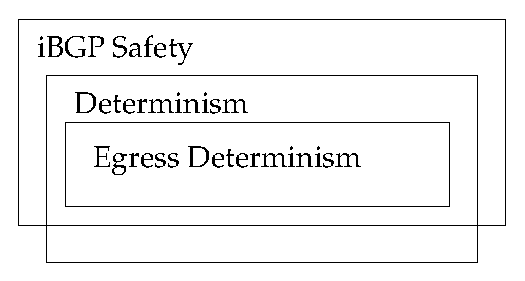
\includegraphics{rlogic/figures/det_venn.eps}}
\end{psfrags}
%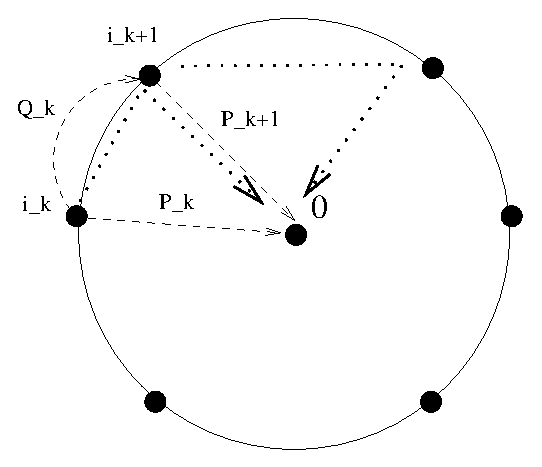
\epsfig{file=policy/figures/dw.eps,width=0.28\textwidth}
\caption[The relationship between determinism, egress determinism, and
  safety.]{The relationship between determinism, egress determinism, and
  safety.} 
\label{fig:determinism_venn}
\end{figure}


\begin{defn}[Egress Determinism]\label{def:egress_determinism}
Let $E_d$ be the set of routes for destination $d$ learned at {\em any}
router in the AS.  Then, a routing protocol satisfies {\em egress
determinism} for destination $d$ if $\lambda_r(E_d)$ satisfies the
following two properties:
\begin{enumerate}
\itemsep=-1pt
\item $\lambda_r(E_d) = \lambda_r(E'_d)$, where $E'_d$ is any subset of
  $E_d$ that contains $\lambda_r(E_d)$, and
\item $\lambda_r(E_d)$ does not depend on the order in which the routes
  in $E_d$ arrived at router $r$.
\end{enumerate}
\end{defn}

\begin{figure}
\centering
\begin{psfrags}
%
\psfrag{x}{{\LARGE $x$}}
\psfrag{y}{{\LARGE$y$}}
\psfrag{z}{{\LARGE $z$}}
\psfrag{X}{{\LARGE $X$}}
\psfrag{Y}{{\LARGE $Y$}}
\psfrag{Z}{{\LARGE $Z$}}
\psfrag{R1}{{\LARGE $R_1$}}
\psfrag{R2}{{\LARGE $R_2$}}
%
%\hspace{-0.7in}
\resizebox{0.6\textwidth}{!}{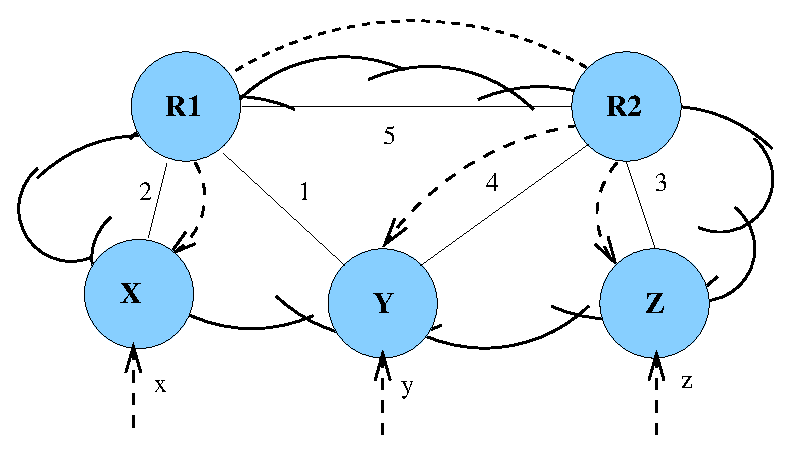
\includegraphics{rlogic/figures/det_violation_rr.eps}}
\end{psfrags}
%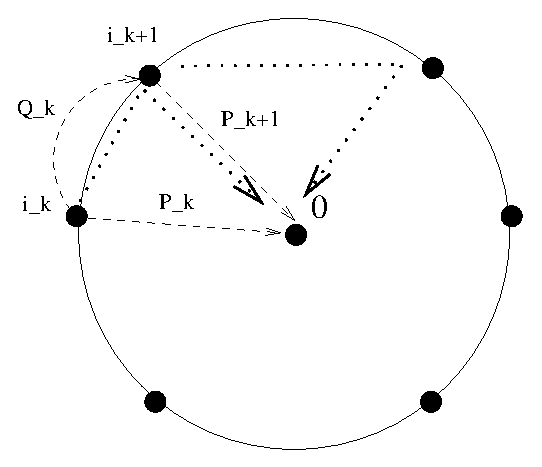
\epsfig{file=policy/figures/dw.eps,width=0.28\textwidth}
\caption[The interaction of IGP and iBGP can cause a violation of egress
  determinism.]{The interaction of IGP and iBGP can cause a violation of egress
  determinism. $\lambda_{R_1}$ is equal to either $x$ or $y$ depending
  on whether $z \in E_d$.}
\label{fig:det_violation_rr}
\end{figure}

Note that egress determinism is a stronger condition than determinism
because it states
properties that $\lambda_r$ must satisfy over the set of routes learned
by all routers in the AS, not just the routes learned at $r$.

If every router in the AS always learned all routes in $E_d$, then
violations of egress determinism would never cause oscillations: given a
fixed set of routes $E_d$, every router would always see that set and
select the same route.  In an iBGP topology with route reflectors,
however, most routers will see some subset of $E_d$, which means that
violations of egress determinism may cause safety violations.  Consider
Figure~\ref{fig:det_violation_rr}: $X$ is a route reflector client of
$R_1$, and $Y$ and $Z$ are clients of route reflector $R_2$. Suppose
that routers $X$, $Y$, and $Z$ all learn routes for some destination $d$
with equal local preference, AS path length, origin type, and MED
attributes, causing routers within the pictured AS to resort to
preferring eBGP routes over iBGP routes, and, that being equal, to
prefer routes with the shortest IGP path cost.  If $E_d = \{x,y,z\}$,
then $\lambda_{R_1}(E_d) = x$: $R_2$ selects $z$ due to its shorter IGP
path cost to the next hop, and $R_1$, having learned $x$ and $z$,
selects route $x$.  If, on the other hand, $E_d = \{x,y\}$, then
$\lambda_{R_1}(E_d) = y$: $R_2$ selects $y$, and $R_1$, having learned
both $x$ and $y$, selects $y$ due to the shorter IGP path cost. Thus,
the first condition of egress determinism is violated.

\begin{figure}
\centering
\begin{psfrags}
%
\psfrag{R1}{{\LARGE $R_1$}}
\psfrag{R2}{{\LARGE $R_2$}}
\psfrag{R3}{{\LARGE $R_3$}}
\psfrag{x}{{\LARGE $x$}}
\psfrag{y}{{\LARGE $y$}}
\psfrag{z}{{\LARGE $z$}}
\psfrag{r1}{{\LARGE $\lambda_{R_1}(\{x,y\}) = y$;
    $\lambda_{R_1}(\{x,y,z\}) = x$}}
\psfrag{r2}{{\LARGE $\lambda_{R_2}(\{x,z\}) = z$;
    $\lambda_{R_2}(\{x,y,z\}) = x$}} 
\psfrag{r3}{{\LARGE $\lambda_{R_3}(\{y,z\}) = z$;
    $\lambda_{R_3}(\{x,y,z\}) = y$}}
\psfrag{x/y}{{\LARGE $x/y$}}
\psfrag{y/z}{{\LARGE $y/z$}}
\psfrag{x/z}{{\LARGE $x/z$}}
%
\hspace{-0.7in}
\resizebox{0.85\textwidth}{!}{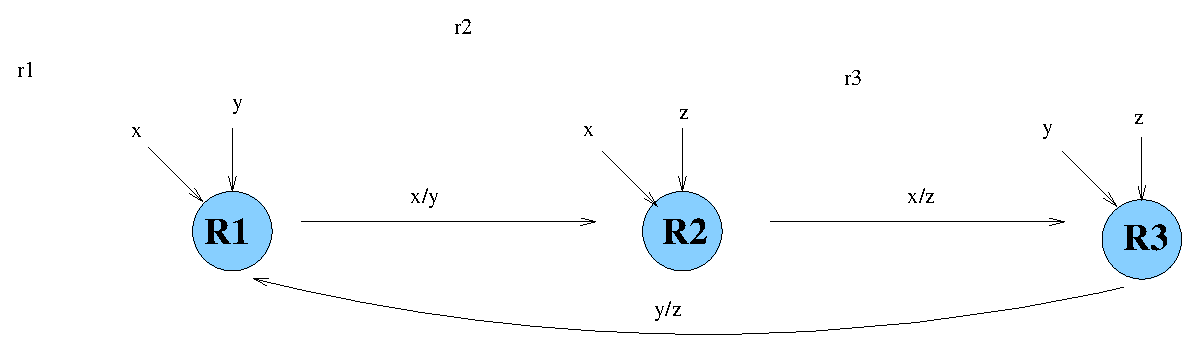
\includegraphics{rlogic/figures/abstract_sd.eps}}

\end{psfrags}
%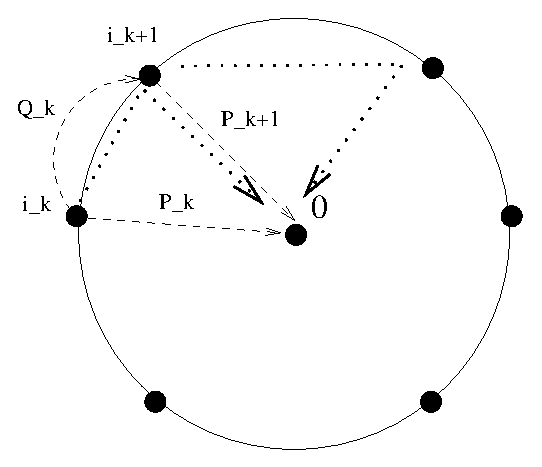
\epsfig{file=policy/figures/dw.eps,width=0.28\textwidth}
\caption[Egress determinism violations can cause safety
  violations.]{Violations of egress determinism can also cause the
  routing protocol to violate safety.}
\label{fig:abstract_sd}
\end{figure}


Like determinism violations, egress determinism violations can cause the
routing protocol to violate safety.  Consider three routers whose
selection functions violate egress determinism, as shown in
Figure~\ref{fig:abstract_sd}; $R_1$'s selection function is identical to
that in Figure~\ref{fig:det_violation_rr}. Each router prefers one route
or the other depending on the presence or absence of a third route.  In
this case, there is no stable assignment of routes $x$, $y$, and $z$ to
routers $R_1$, $R_2$, and $R_3$.  For example, if $R_1$ selects $x$,
then $R_2$ selects $z$ and $R_3$ selects $y$, prompting $R_1$ to select
$y$, and so on.  This very scenario can be realized in BGP today if
three routers' route selection functions fail to satisfy egress
determinism, as shown in Figure~\ref{fig:sd_violation_rr_osc}.


\begin{figure}[t]
\centering
\begin{psfrags}
%
\psfrag{x}{{\LARGE $x$}}
\psfrag{y}{{\LARGE$y$}}
\psfrag{z}{{\LARGE $z$}}
\psfrag{X}{{\LARGE $X$}}
\psfrag{Y}{{\LARGE $Y$}}
\psfrag{Z}{{\LARGE $Z$}}
\psfrag{R1}{{\LARGE $R_1$}}
\psfrag{R2}{{\LARGE $R_2$}}
\psfrag{R3}{{\LARGE $R_3$}}
%
%\hspace{-0.7in}
\resizebox{0.6\textwidth}{!}{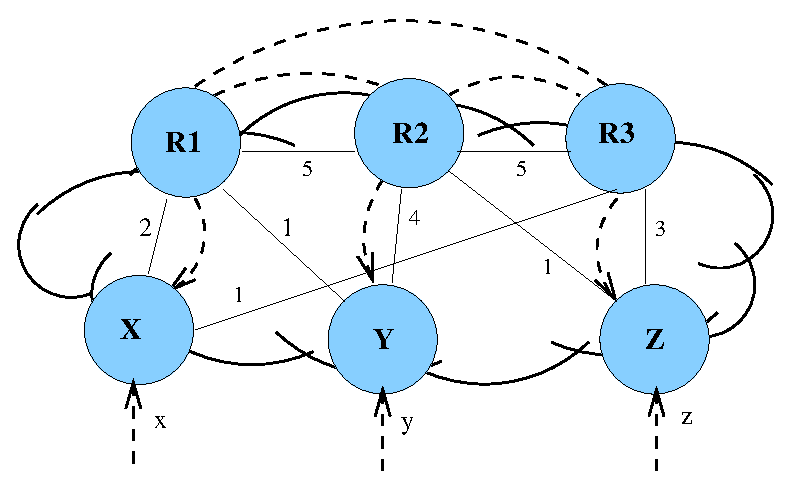
\includegraphics{rlogic/figures/sd_violation_rr_osc.eps}} 

\end{psfrags}
%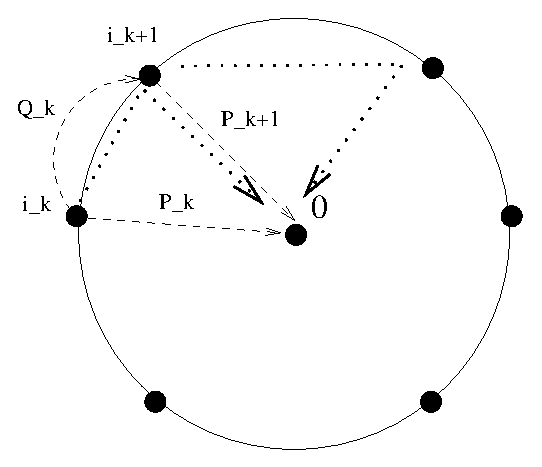
\epsfig{file=policy/figures/dw.eps,width=0.28\textwidth}
\caption[The interaction of IGP and iBGP can cause a violation of egress
  determinism.]{The interaction of IGP and iBGP can cause a violation of egress
  determinism that induces a safety violation.  This figure shows the
  instantiation of Figure~\ref{fig:abstract_sd} in BGP.  Previous work has
  also observed that violations of this type could occur~\cite{Griffin2002}
  but did not observe that these could be constructed in general by
  composing egress determinism violations.}
\label{fig:sd_violation_rr_osc}
\end{figure}


\begin{figure}
\begin{center}
\begin{psfrags}
\psfrag{R1}{{\LARGE $R_1$}}
\psfrag{R2}{{\LARGE $R_2$}}
\psfrag{X}{{\LARGE $X$}}
\psfrag{Y}{{\LARGE $Y$}}
\psfrag{Z}{{\LARGE $Z$}}
\psfrag{x}{{\Large $x$}}
\psfrag{y}{{\Large $y$}}
\psfrag{z}{{\Large $z$}}
\psfrag{l1}{{\Large $l_r$}}
\psfrag{ly}{{\Large $l_y$}}
\psfrag{lx}{{\Large $l_x$}}
\psfrag{lz}{{\Large $l_z$}}
\resizebox{0.45\textwidth}{!}{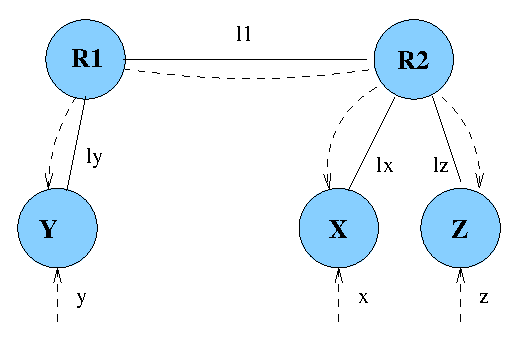
\includegraphics{rlogic/figures/det_igp.eps}}
\end{psfrags}
\end{center}
\caption[The main idea of the proof of
  Lemma~\ref{lem:det_igp}.  ]{The main idea of the proof of
  Lemma~\ref{lem:det_igp}.  
%
If $R_2$ prefers $z$ over $x$, then $l_z \leq l_x$.
%
If $R_1$ prefers $x$, given routes $x$, $y$, and $z$, then $l_y \geq
  l_r + l_x$.  If $R_2$ is on the shortest IGP path between $R_1$ and
  both $X$ and $Z$, it follows that $l_y \geq l_r + l_z$ (and, hence,
  $R_1$ would {\em not} have selected route $y$).  Thus, for $R_1$ to
  prefer route $y$ when it learns routes $x$ and $z$, its shortest path
  to either egress router $Y$ or $Z$ must not traverse $R_2$. (The links
  labeled with $l_x$, $l_y$, and $l_z$ are shown as single IGP links,
  but the argument generalizes to IGP paths.)}
\label{fig:det_igp}
\end{figure}



\begin{lemma}\label{lem:det_igp}
If an AS's iBGP topology is {\em RR-IGP-Consistent}, and every router's
selection function satisfies determinism, then every router's selection
function also satisfies egress determinism.
\end{lemma}

\begin{proof}
Suppose that there exists some router $R_1$ and routes $x$, $y$, and $z$
(not necessarily learned via eBGP at $R_1$) such that
$\lambda_{R_1}(\{x,y,z\}) = y$, but $\lambda_{R_1}(\{x,y\}) = x$.  
%
First, because $\lambda_{R_1}$ satisfies determinism, it must be the case
that (1)~$R_1$ learns $x$ via iBGP and (2)~some router $R_2$ in the iBGP
topology withdraws the eBGP-learned 
route $x$ from router $R_1$ upon learning the route $z$, thereby
preventing router $R_1$ from receiving route $x$ (if $R_1$ had learned
$x$ directly via eBGP, it would continue to select route $x$).
%
Second, $R_2$ must have selected $z$ over $x$ because it had a shorter
IGP path to the router from which it learned $z$---if $x$ had been less
desirable based on some other attribute (\eg, AS path length), then $r$
would have also selected the route $z$ upon learning it from $R_2$,
rather than selecting $y$ instead.
%
Third, because $R_1$ selects $y$ after learning $z$ from $R_2$, its IGP
path to the egress router that learned $y$ must be shorter than its IGP
path to the router that learned $z$, yet longer than its IGP path to the
router that learned $x$.   
%
This relation among distances to egresses is only possible if the
shortest path between $R_1$ and either the egress router that learned
route $x$ or $z$ does not traverse $R_2$ (\ie, the iBGP topology is not
{\em RR-IGP-Consistent}).  Figure~\ref{fig:det_igp} shows why this
relation is not possible in an iBGP topology that is {\em
RR-IGP-Consistent}.
\end{proof}

We now state the conditions for iBGP to satisfy safety using our results
involving determinism and egress determinism.  Specifically, we show
that if MED is compared across all routes (\ie, every router's selection
function satisfies determinism) and if the iBGP topology is {\em
RR-IGP-Consistent} (\ie, egress determinism is satisfied), then iBGP
satisfies safety.

\begin{figure}
\begin{center}
\begin{psfrags}
\psfrag{R1}{{\LARGE $R_1$}}
\psfrag{R2}{{\LARGE $R_2$}}
\psfrag{C1}{{\LARGE $C_1$}}
\psfrag{C2}{{\LARGE $C_2$}}
\resizebox{0.55\textwidth}{!}{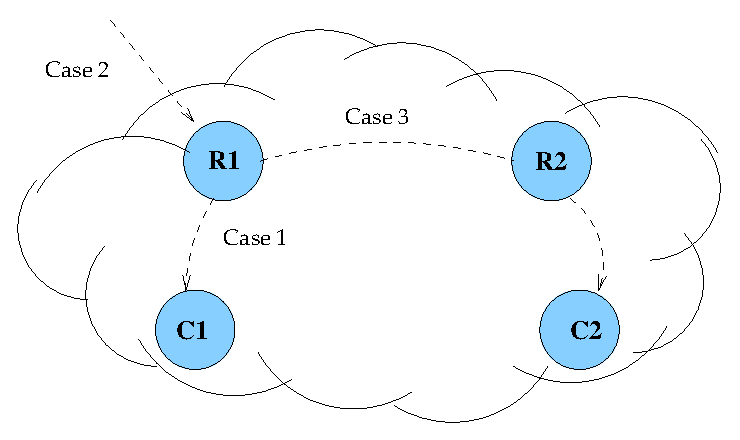
\includegraphics{rlogic/figures/always_compare.eps}} 
\end{psfrags}
\end{center}
\caption[The three cases in the proof of
  Theorem~\ref{th:always_compare}.]{The three cases in the proof of
  Theorem~\ref{th:always_compare}.}
\label{fig:always_compare}
\end{figure}



\begin{theorem}\label{th:always_compare}
If every router's selection function compares MED attribute across all
routes and the iBGP topology is {\em RR-IGP-Consistent}, then iBGP
satisfies safety.
\end{theorem}

\begin{proof}
The proof follows from Lemmas~\ref{lem:det_med} and~\ref{lem:det_igp}.
If the conditions of the theorem hold, then BGP satisfies both
determinism and egress determinism.  It remains to show that no iBGP
topology can violate safety if it satisfies both determinism and egress
determinism.  

We must show that, for any route that a router ultimately selects, other
routers in the AS will not select routes that ultimately causes the
original router to change the route it selects.  For simplicity, we will
consider an iBGP route reflector hierarchy with one level.  The argument
can be extended to a multiple-level hierarchy, and to a network with
multiple top-level routers or multiple clients per route reflector,
without loss of generality.  Consider the possible propagation of BGP
routes between routers $C_1$ and $C_2$ and their route reflectors $R_1$
and $R_2$, as shown in Figure~\ref{fig:always_compare}.  Suppose $C_1$
and $C_2$ initially select routes via eBGP; each will readvertise these
routes to $R_1$ and $R_2$.  Then, there are three cases:

\begin{enumerate}
\itemsep=-1pt
\item {\em $R_1$ prefers the route through its client $C_1$.}
In this case, $R_1$'s selection of the route through $C_1$ will
obviously not cause either $R_1$ or $C_1$ to switch paths.  
%
\item {\em $R_1$ prefers its own eBGP-learned route (analogously for
$R_2$).}  In this case, $C_1$ learns a route via $R_1$. If it
continues to prefer its own route, neither router will select a new
route. If, on the other hand, it prefers the route through $R_1$, then
it will withdraw its eBGP-learned route from $R_1$.  However, since
$\lambda_{R_1}$ satisfies determinism, $R_1$ will continue to select its
own eBGP-learned route when it receives this withdrawal.
%
\item {\em $R_1$ prefers a route via $R_2$ or $C_2$ (analogously for
$R_2$).}  A similar argument can be used to show that
neither $R_1$ nor $C_1$ will select a new route once $R_1$ selects a
route via $C_1$.  For the third case, we must also show that $R_1$'s
withdrawal of either its own route or the route via $C_1$ from $R_2$
will cause neither $R_2$ nor $C_2$ to change routes.  Since $R_1$
prefers a route via $R_2$ then $R_2$ selected its own route
or the route via $C_2$; egress determinism guarantees that $R_1$'s
withdrawal will not cause either $C_2$ or $R_2$ to change its route
selection.
\end{enumerate}
\end{proof}

Our definitions have allowed us to derive sufficient
conditions on safety that are significantly weaker (and therefore, the
result is stronger) than in
previous work~\cite{Griffin2000}.  In particular, {\em our results show
that assuming that the relationships between route reflectors and their
clients are acyclic is unnecessary} (although a cyclic topology may make
an oscillation more likely if egress determinism is
violated).  It turns out that the only way for a cyclic iBGP topology
to cause oscillations would be for either the iBGP topology to not be
{\em RR-IGP-Consistent} or for some IGP edges to have
negative edge weights.

\begin{figure}
\centering
\begin{psfrags}
%
\psfrag{x}{{\LARGE $x$}}
\psfrag{y}{{\LARGE$y$}}
\psfrag{z}{{\LARGE $z$}}
\psfrag{X}{{\LARGE $X$}}
\psfrag{Y}{{\LARGE $Y$}}
\psfrag{Z}{{\LARGE $Z$}}
\psfrag{R1}{{\LARGE $R_1$}}
\psfrag{R2}{{\LARGE $R_2$}}
\psfrag{R3}{{\LARGE $R_3$}}
\psfrag{l1}{{\LARGE $l_1$}}
\psfrag{l2}{{\LARGE $l_2$}}
\psfrag{l3}{{\LARGE $l_3$}}
\psfrag{l4}{{\LARGE $l_4$}}
\psfrag{l5}{{\LARGE $l_5$}}
\psfrag{l6}{{\LARGE $l_6$}}
%
%\hspace{-0.7in}
\resizebox{0.7\textwidth}{!}{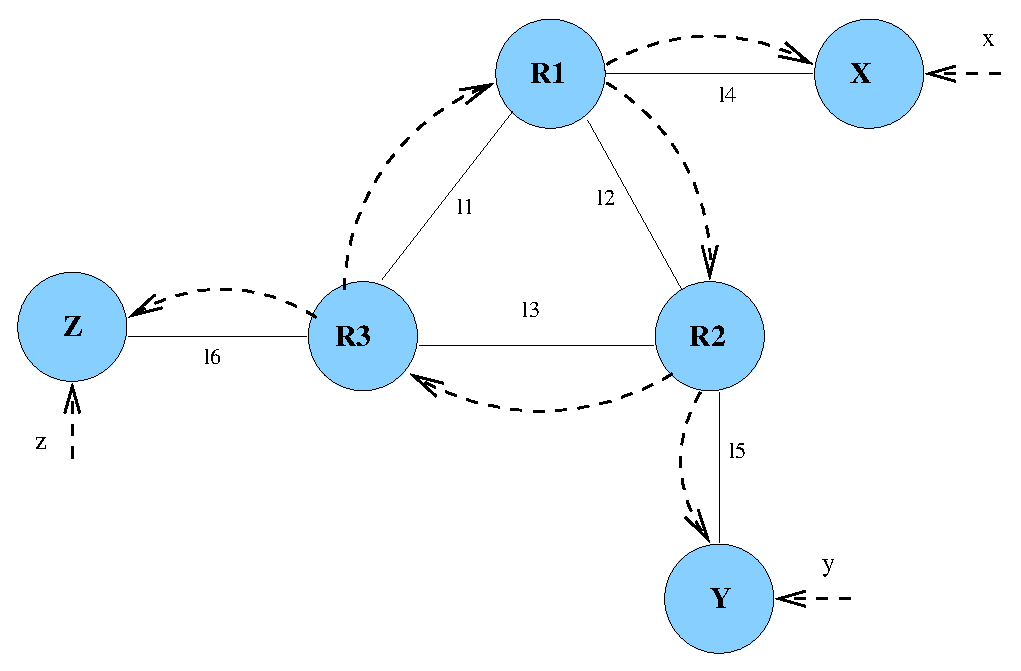
\includegraphics{rlogic/figures/ibgp_cycle.eps}} 

\end{psfrags}
%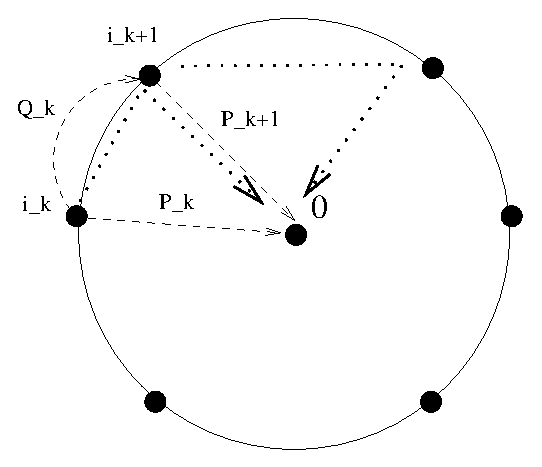
\epsfig{file=policy/figures/dw.eps,width=0.28\textwidth}
\caption[When iBGP satisfies egress determinism,
  a cyclic iBGP topology typically do not cause safety violations.]{When iBGP
  violates safety but satisfies egress determinism, the only way a
  cyclic iBGP topology can 
  violate safety is if the IGP allows negative edge weights.  This
  example shows an iBGP hierarchy that includes only six routers, but it
  generalizes: $R_i$ could be any cyclic relationship at the top of the
  hierarchy, $X$ could be a path through a sequence of iBGP sessions to
  the egress router $X$ (\eg, a sequence of route reflector-client
  sessions) and $l_4$ could be the cost of that path, and so forth.}
\label{fig:ibgp_cycle}
\end{figure}



To understand why cycles in the iBGP hierarchy do not cause problems if
the topology is {\em 
RR-IGP-Consistent}, see Figure~\ref{fig:ibgp_cycle}.  In this example,
if egress determinism is satisfied, then the only case where an
oscillation might result is where $R_1$ prefers route $y$ over route
$x$, $R_2$ prefers route $z$ over $y$, and $R_3$ prefers $x$ over $z$.
All other cases where oscillation might occur (\ie, those caused by
violations of egress determinism) require some shortest IGP path between
a router and another egress to not traverse that router's route reflector.
For safety to be violated in this example, routes $x$, $y$, and $z$ must
all have equal local preference, AS path length, origin type and MED
(otherwise, all routers would select the most preferable route or
routes).  Presuming that all routes are equally good up to the step in
route selection involving the IGP tiebreak, then the only way for such a
situation to occur is if the following inequalities were satisfied:
\begin{eqnarray*}
l_1 + l_4 & < & l_6 \\
l_2 + l_5 & < & l_4 \\
l_3 + l_6 & < & l_5 
\end{eqnarray*}
which implies that $l_1 + l_2 + l_3 < 0$, or that some IGP edge weights
must be negative.

Theorem~\ref{th:always_compare} is significant because
the conditions on the iBGP topology that are required to guarantee
safety are identical those for guaranteeing route validity, as stated in
Theorem~\ref{th:rr_safe}.  Furthermore, because there are now known
techniques for {\em generating} these
configurations~\cite{Vutukuru2005}, our results are prescriptive, since
this technique that was designed to generate iBGP topologies that
guarantee route validity also happens to generate topologies that
guarantee safety.

This section has described safety violations that result from
protocol interactions {\em within a single AS}.  However, safety is a somewhat
unique property because it inherently depends on how different ASes are
allowed to rank candidate routes to a destination (\ie,
Observation~\ref{obs:composable} is not satisfied).  Whereas, in iBGP, a
router's rankings are constrained by the underlying IGP
topology, in eBGP, an AS's rankings can be arbitrary.
Verifying a property that involves analyzing the interactions
between the configurations of multiple ASes is challenging:
because these ASes compete with one another, no single AS has knowledge 
of the configurations of other ASes.  Chapter~\ref{chap:policy} explores
how safety can be guaranteed {\em across multiple ASes} without
requiring each AS to expose its configurations to other ASes.


\section{Summary}

Detecting problems in Internet routing requires a precise
specification of correct behavior and a framework for reasoning about
whether that specification is satisfied.  In this chapter, we presented
a three-part correctness specification: route validity, path visibility,
and safety. We explained why each of these properties is important for the
fundamental operation of Internet routing and reasoned about how these
properties may be satisfied or violated in the context of BGP.

In the subsequent chapters of this dissertation, we will use the
specification constraints to guide the operations and design of correct
Internet routing.  In Chapter~\ref{chap:rcc}, we will explore how static
configuration analysis can be used to guarantee that two of these
properties---route validity and path
visibility---hold. 
Theorems~\ref{th:mesh}--\ref{thm:vis}
%, \ref{th:rr_safe},
%\ref{th:mesh_visibility}
%, and~\ref{thm:vis} 
suggest invariants on
configuration that could be verified by detecting when the configuration
violates certain invariants, and both Theorem~\ref{th:always_compare}
and the discussion at the end of
Section~\ref{sec:mesh}
suggest possible protocol modifications.  In
Chapter~\ref{chap:sandbox}, we will exploit the fact that, when the
routing protocol satisfies certain aspects of this specification
(specifically, path visibility, safety, and, in some cases,
determinism), we can design algorithms that efficiently predict the
routes that each router in an AS will ultimately select.
Chapter~\ref{chap:policy} tackles the problem of guaranteeing safety in
the context of eBGP, which is challenging since it inherently involves
dependencies between the policies of multiple independent (and often
competing) ASes.
%Chapter~\ref{chap:beyond} explores how both analysis of
%routing protocol dynamics and modifications to the routing architecture
%itself can complement static configuration analysis.

